%\documentclass[3p,twocolumn]{elsarticle}
\documentclass[review]{elsarticle}
\usepackage{graphicx}
\usepackage[export]{adjustbox}%for left right graphic adjust
\usepackage{amsmath}
\usepackage{float}
\graphicspath{ {images/} }

\usepackage{lineno,hyperref}
\modulolinenumbers[5]

\journal{Journal of \LaTeX\ Templates}

%%%%%%%%%%%%%%%%%%%%%%%
%% Elsevier bibliography styles
%%%%%%%%%%%%%%%%%%%%%%%
%% To change the style, put a % in front of the second line of the current style and
%% remove the % from the second line of the style you would like to use.
%%%%%%%%%%%%%%%%%%%%%%%

%% Numbered
%\bibliographystyle{model1-num-names}

%% Numbered without titles
%\bibliographystyle{model1a-num-names}

%% Harvard
%\bibliographystyle{model2-names.bst}\biboptions{authoryear}

%% Vancouver numbered
%\usepackage{numcompress}\bibliographystyle{model3-num-names}

%% Vancouver name/year
%\usepackage{numcompress}\bibliographystyle{model4-names}\biboptions{authoryear}

%% APA style
%\bibliographystyle{model5-names}\biboptions{authoryear}

%% AMA style
%\usepackage{numcompress}\bibliographystyle{model6-num-names}

%% `Elsevier LaTeX' style
\bibliographystyle{elsarticle-num}
%%%%%%%%%%%%%%%%%%%%%%%

\begin{document}

\begin{frontmatter}

%\title{Extending Dynamic Range of Generic Electronics for Time Projection Chambers (GET)}
\title{Extending the Dynamic Range of Electronics in a Time Projection Chamber}
%\title{Extending Dynamic Range of GET Electronics}

%% Group authors per affiliation:
%\author{Elsevier\fnref{myfootnote}}
%\address{Radarweg 29, Amsterdam}
%\fntext[myfootnote]{Since 1880.}

%% or include affiliations in footnotes:
\author[msu,nscl]{J. Estee}
\author[msu,nscl]{W.G. Lynch}
\author[msu,nscl]{J. Barney}
\author[msu,nscl]{G. Cerizza}
\author[kor]{B. Hong}
\author[riken]{T. Isobe}
\author[nscl]{G. Jhang}
\author[kyoto]{M. Kaneko}
\author[riken]{M. Kurata-Nishimura}
\author[krakow]{P. Lasko}
\author[kor]{J. W. Lee}
\author[krakow]{J. Lukasik}
\author[a&m]{A.B. McIntosh}
\author[kyoto]{T. Murakami}
\author[krakow]{P. Pawlowski}
\author[poland]{K. Pelczar}
\author[nscl]{C. Santamaria}
\author[riken]{D. Suzuki}
\author[nscl]{M. B. Tsang}
\author[a&m]{S.J. Yennello}
\author[tsing]{Y. Zhang}
\author[]{and the S$\pi$RIT collaboration}

\address[msu]{Michigan State University, Dept. Physics and Astronomy }
\address[nscl]{National Superconducting Cyclotron Laboratory}
\address[kor]{Department of Physics, Korea University}
\address[riken]{RIKEN Nishina Center}
\address[kyoto]{Department of Physics, Kyoto University}
\address[krakow]{IFJ PAN, Krak\'{o}w}
\address[a&m]{Dept. of Physics and Astronomy, Texas A$\&$M University}
\address[tsing]{Department of Physics, Tsinghua University}
\address[poland]{Faculty of Physics, Astronomy and Applied Computer Science, Jagiellonian University}



\begin{abstract}
As Time Projection Chambers (TPCs) become widely used in low to intermediate nuclear physics experiments,  it becomes important to extend the dynamic range to cover  the large range in energy losses. In a recent set of experiments using the SAMURAI Pion-Reconstruction and Ion-Tracker (S$\pi$RIT) TPC, it was important to simultaneously measure relativistic pions and heavy ions from the same collisions. A track which saturates the TPC electronics only does so for several pads near to the track while pads further away are not saturated. By performing a $\chi^2$ fit using the pad response function on the unsaturated pads, we can recover the saturated pad's charges. This resulted in an increase of the dynamic range by a factor of 2. 
\end{abstract}

\begin{keyword}
\texttt{elsarticle.cls}\sep \LaTeX\sep Elsevier \sep template
\MSC[2010] 00-01\sep  99-00
\end{keyword}

\end{frontmatter}

\linenumbers

\section{Introduction} 
 At low to intermediate heavy ion collision (HIC) energies, it may be necessary to measure particles that have a large variation in energy losses. At the time of publication it is common for Time Projection Chamber (TPC) electronics to have a dynamic range, the maximum signal to noise ratio, of around 1000:1. If a signal to noise ratio of at least 20:1 is required to measure minimum ionizing particles (m.i.p.), around $\beta\gamma=0.4$, this means the maximum range we could expect would be 50x greater than m.i.p.  In heavy ion collisions (HIC) of 300 AMeV beam energies the range of particle velocities ranges from m.i.p. to ~0.1$\beta\gamma$. These velocities alone cover about 40x the dE/dx of m.i.p. Since the energy loss scales like $z^2$ for larger charged particles we could expect a factor of 9x more for z=3 charged particles. Also, if the track enters the TPC at an obtuse angle, the collected charge on one pad could be higher by a factor of about 4x.  It becomes clear the large dynamic range that must be covered in such intermediate HIC experiments. 
 
 \begin{figure}[H]
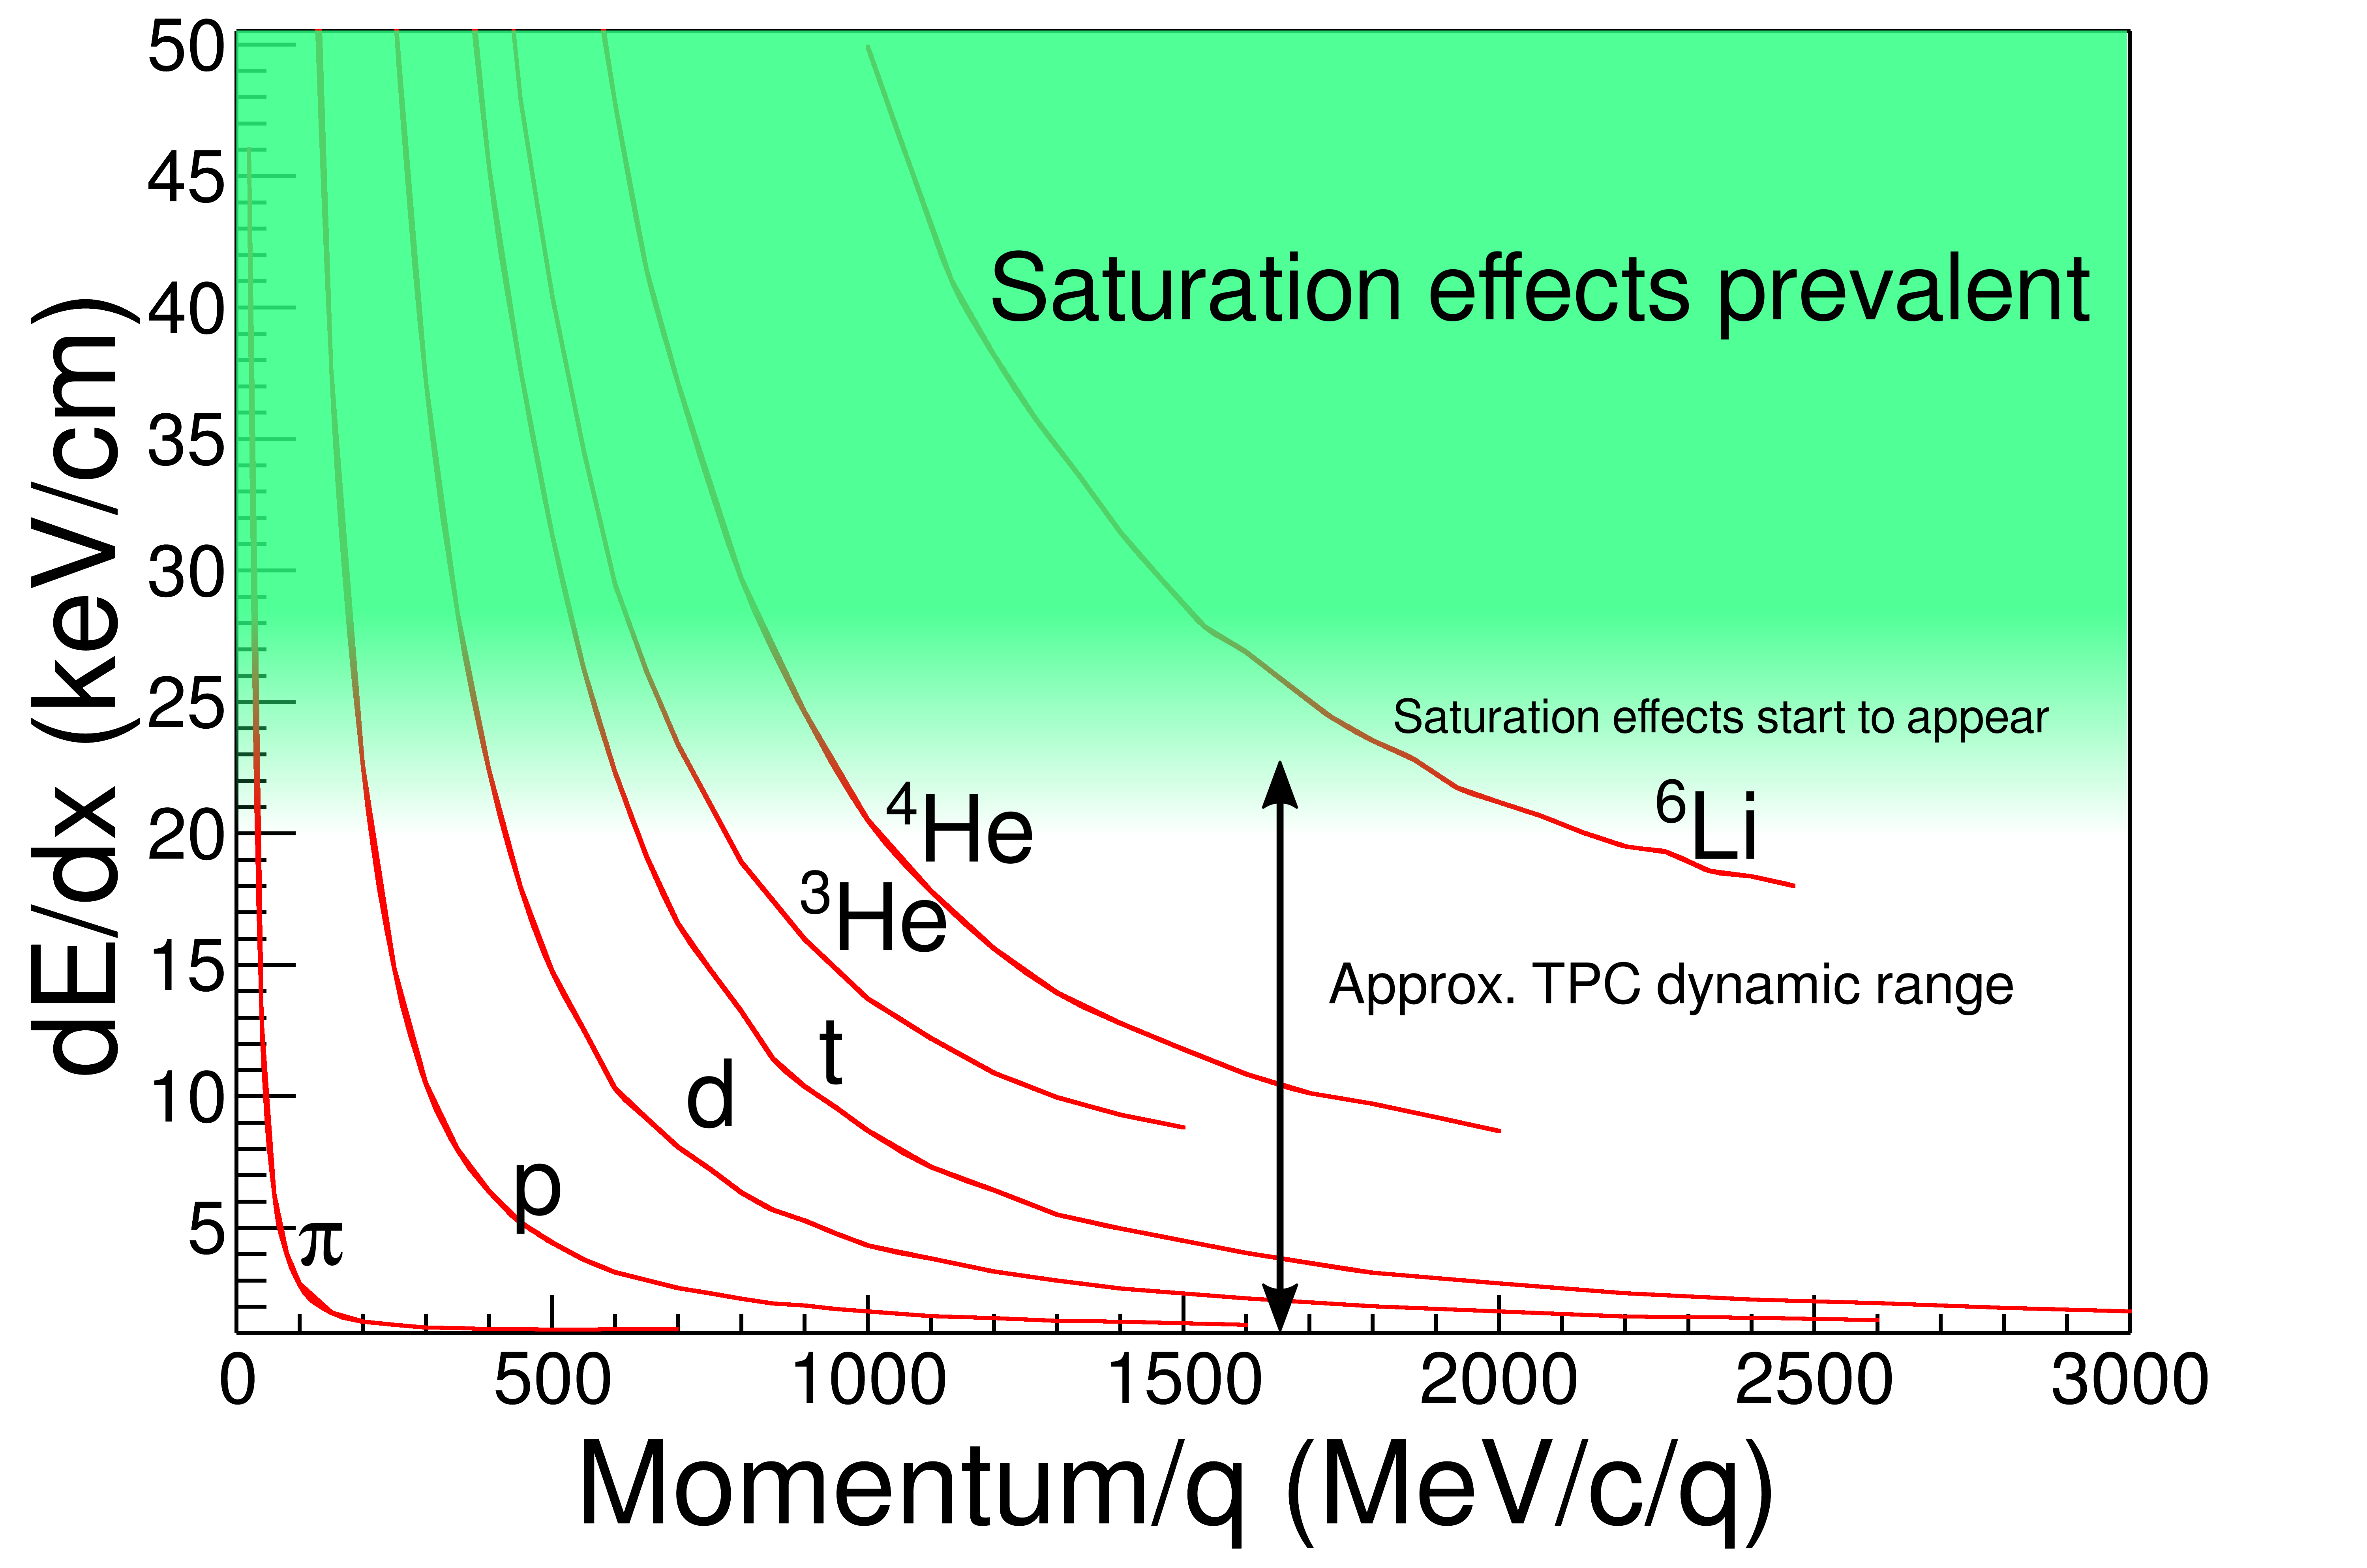
\includegraphics[width=\linewidth]{intrographic}
\caption{}
\label{fig:intro}
\end{figure}

Several techniques have been employed to address this issue in TPCs. A couple of TPCs such as the EOS TPC \cite{eos} or the AT-TPC were able to circumvent the measuring of large energy deposits by lowering the gain in certain regions either by lowering the voltage on the anode wires or electronics gain settings. Lowering the gain in large regions of the TPC worsens the dE/dx resolution and momentum determination for m.i.p. as only a subset of the whole TPC can be used. Also there may be no dE/dx measurement for tracks that avoid these regions. Here we illustrate how to expand the dynamic range without these drawbacks within the context of a standard multi-wire TPC. 




\begin{figure}[H]
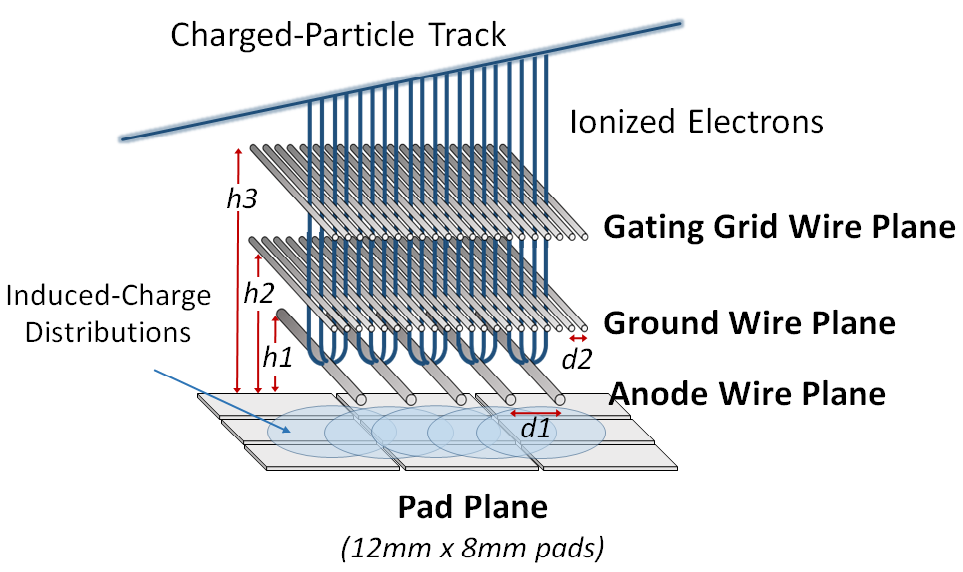
\includegraphics[width=\linewidth]{padwire}
\caption{Cartoon graphic showing the 3 wire planes and a section of the pad plane. h3 =14 mm, h2 = 8 mm, h1 = 4 mm, d2 = 1 mm, d1 = 4 mm. This graphic is inverted from the actual wire planes and pad plane to display the perspective easier.}
\label{fig:padwire}
\end{figure}

\paragraph{1.1 TPC Overview}
\paragraph{Wire planes}
As seen in figure \ref{fig:padwire} the S$\pi$RIT TPC consists of three wire grids below the two dimensional array of charge sensitive readout pads, the pad plane. The first two wire grids operate as a gate and a shielding, or ground grid, with 1 mm spacing and they are not important for the discussion of this paper. The wire grid closest to the pad plane is the high voltage anode wire grid consisting of 20 $\mu$m wires spaced at 4 mm apart and set at a height of 4 mm from the pad plane. In the near vicinity of these wires the avalanche of the preliminary electrons occurs. The electrons deposited from tracks in the detector gas are multiplied on the order of 2000  times and the slow moving ions induce a signal on the read out pads below. The resulting distribution on the pad plane is fixed by the geometry of the anode wire grid and its distance from the pad plane. The anode wire planes were sectioned off into 14 independent sections. 12 sections of the anode wire planes were held at 1460 V. This setting was optimized to ensure the small signal of pions would at have a least a signal to noise ratio of 20:1. Two of the sections were held to 1214 V due to a concern of the current each section was drawing. The reduction in voltage resulted in a reduction in gain of about 10x compared to the higher anode wire sections. These two sections of lower gain allowed for a direct validation of the method that will be described. 



\paragraph{Pad plane} 
The S$\pi$RIT TPC pad plane consists of a 2-dimensional plane of charge sensitive pads which are rectangular in shape with a dimension of 0.8 cm x 1.2 cm. It is laid out on a grid measuring 112 by 108 pads with a total area of 134 cm x 86 cm. For convenience we have chosen the +x axis to point to the left of beam, the -y axis as the direction pointing down into the drift volume, and the +z axis along the incoming beam. The avalanche wires run perpendicular to the beam axis along the x axis as seen in the figure \ref{fig:padwire}. 
\paragraph{Generic Electronics for TPCs}
Signals from the pads in the S$\pi$RIT TPC are amplified and digitized by the newly developed Generic Electronics for TPCs (GET) \cite{get}.  Short cables transmit the signals from the pads to the inputs of the AGET chips. Each AGET chip can service 64 pads and contains a Preamp (PA), and a Switched Capacitor Array (SCA) with a maximum of 512 time buckets sampling at 1 to 100 MHz. Four AGET chips are mounted on one AsAd (Asic and Adc) motherboard. The gain of each AGET can be configured as 0.12, 0.24, 1.0, or 10 pC over the whole dynamic range. Also the peaking times of the shaping amplifiers can be set to 69, 117, 232, 501, 720, or 1014 ns. The ADCs on the AsAd boards deliver a 12 bit resolution. For the first series of experiments the gain was set to the highest setting, 0.12 pC, and the peaking time was set to 117 ns, and the sampling time set to 25 MHz. At such a high gain, the pion signal was able to fully be measured. To put this gain setting into perspective, the minimum velocity that would cause saturated pads was $\beta\gamma\approx$ 0.2 for z=1 particles, $\beta\gamma\approx$ 0.6 for z=2 particles, and z$\geq$3 particles were always saturating. 

\section{Pad Response Function}
\paragraph{Experimental PRF}
When electrons terminate on the anode wires they induce a 2-dimensional charge distribution on the pad plane. The fractional charge seen by each pad is referred to as the Pad Response Function (PRF). Some simple wire plane geometries have analytical expressions for the PRF which are well studied and may be looked up using a Gatti distribution \cite{blumrol}. When analytic PRFs do not exist, an effective PRF may be calculated from experimental data. We postulate that the PRF is only a function of the total charge deposited on the wire Q and the displacement, $\lambda$, from the mean avalanche position $\bar{x}$.

\begin{figure}[H]
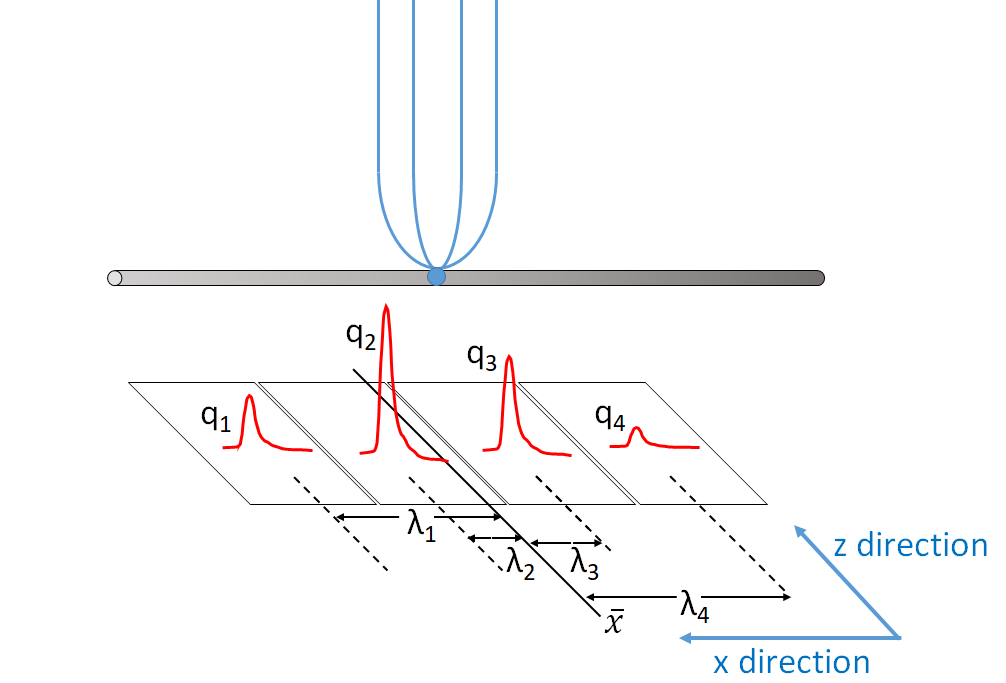
\includegraphics[width=\linewidth]{defofavalanche}
\caption{Cartoon graphic of avalanche event on an anode wire over one layer of pads. The estimate of the position of the avalanche is given by $\bar{x}$  the weighted mean. The position from the center to each pad to the $\bar{x}$ position is given as $\lambda_i$.}
\label{fig:av}
\end{figure}

\begin{equation}\label{eq:1}
\begin{split}
PRF(\lambda_i) = \frac{q_i(\lambda_i)}{Q}\\
where \ Q=\sum_i q_i\\
and \   \lambda_i=x_i-\bar{x}\\
\end{split}
\end{equation}

For the purpose of calculating the effective PRF from experimental data, we selected only the pads which were not saturated. Since the beam comes in along the z direction, the x direction gives the best momentum resolution and was the natural choice for combining hits into clusters and calculating the PRF. 

The way we calculate the PRF is given by equation \ref{eq:1} where i is the index over the pads and Q is the total charge within the layer. Figure \ref{fig:av}  illustrates the estimate for the avalanche position along the wire given by, the weighted mean position $\bar{x}$. Also seen is $\lambda_i$, defined as the difference in position of the center of the $i^{th}$ pad, $x_i$, to the mean position $\bar{x}$. 

\begin{figure}[H]
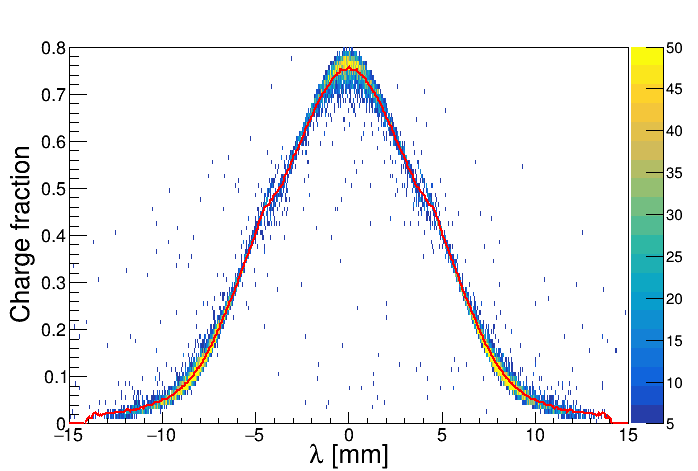
\includegraphics[width=\linewidth]{expprf}
\caption{Experimental pad response function. Constructed from total number of pads $>$=3. }
\label{fig:expprf}
\end{figure}

The resulting experimental PRF for the S$\pi$RIT TPC is shown in figure \ref{fig:expprf} and is obtained from averaging many events and describes a well behaved function. It is this function we will be using to fit the data to extend the saturated pads. 

\paragraph{Method of Desaturaiton}

For convenience we will use the term desaturation for when we estimate and recover the charge values of the saturated pads. Figure \ref{fig:satpad} shows a typical situation of saturated signals. When an avalanche causes a large induced signal, the pads directly underneath collect the largest charge and typically would be saturated. These are represented as $q_{1'}$ and $q_{2'}$ in the figure \ref{fig:satpad}. The pads further away would experience smaller, non-saturated signals shown as $q_{1}$ and $q_{4}$.

Since the charge deposited on each  pad must satisfy the PRF distribution described in figure \ref{fig:expprf}, then using these small non-saturated tails we perform a $\chi^2$ fit to find the unknown charge on the saturated pads. The data points of the $\chi^2$ fit are the unsaturated pads,  $q_{1}$ and $q_{4}$, and the unknown parameters of the fit are $q_{2'}$ and $q_{3'}$ with the expected values coming from the PRF described above. The values of $q_{2'}$ and $q_{3'}$ at the minimum of the $\chi^2$ would be the best estimate for the saturated pads. 

\begin{figure}[H]
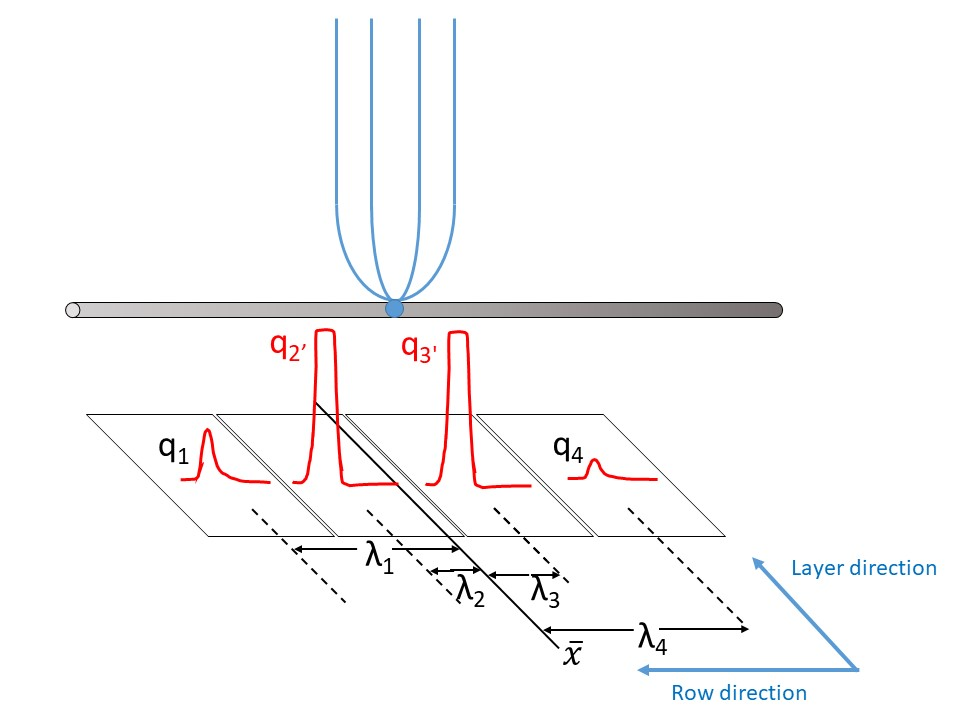
\includegraphics[width=\linewidth]{saturated_pads}
\caption{•}
\label{fig:satpad}
\end{figure}

\section{Experimental data}

Two sets of data were used for testing and validation of this method. The first set was a tuned cocktail beam consisting of (p,d,t,${}^3He$,${}^4He$,${}^6Li$,${}^7Li$) light charged particles which was injected into the TPC for calibration purposes. The cocktail beam was tuned to two different $\beta\rho$ settings and the momentum resolution was approximately 1\% as determined by the slits of the BigRIPS fragment separator of the Radioactive Isotope Beam Factory (RIBF) facility in RIKEN. A thick 21mm thick aluminum target was inserted for part of the lower $\beta\rho$ setting, further reducing the energy of the beam for a third calibration point. 

In a typical cocktail event one particle enters the TPC volume at a time and mostly parallel to the pad plane. Therefore the cocktail beam data represents an ideal case for the momentum and dE/dx determination as it does not suffer from inefficiencies related to high multiplicity events we see in the collision experimental data.  

\begin{figure}[H]
\includegraphics[width=\linewidth]{data.pdf}
\caption{Pad plane projection for a collision event in the TPC. Highlighted by red arrows are two regions of anode wires which had a reduced voltage of 1214 V. The voltage of the rest of the TPC anode wires are 1460 V. The reduction in voltage reduces the gain by a factor of about 10x. }
\label{fig:data}
\end{figure}

The other type of data was where we collided a ${}^{132}$Sn beam onto a ${}^{124}$Sn target in which we triggered on central nuclear collisions. Shown in figure \ref{fig:data} is the typical pad plane response for a central nuclear collision. During the experiment the voltages of two anode sections (as indicated by red arrows in figure \ref{fig:data} were turned down from 1460 V to 1214 V. Since the anode voltages were dropped, the gain of these sections were also reduced by a factor of about 10x. 


\section{Results}
\paragraph{Low gain vs corrected high gain}

As mentioned above two anode sections, covering 12 layers of pads in total, had their gain lowered by approximately a factor of 10x. Thus, the signals in this lowered gain region have effectively 10x the dynamic range as compared with the high gain regions. That is to say when a track would saturate pads in the high gain region, the signal in this low gain region was still preserved and could be measured. By comparing the dE/dx values of the high gain sections with the low gain section we can determine whether the desaturation correction described above is successful. 

\begin{figure}[H]
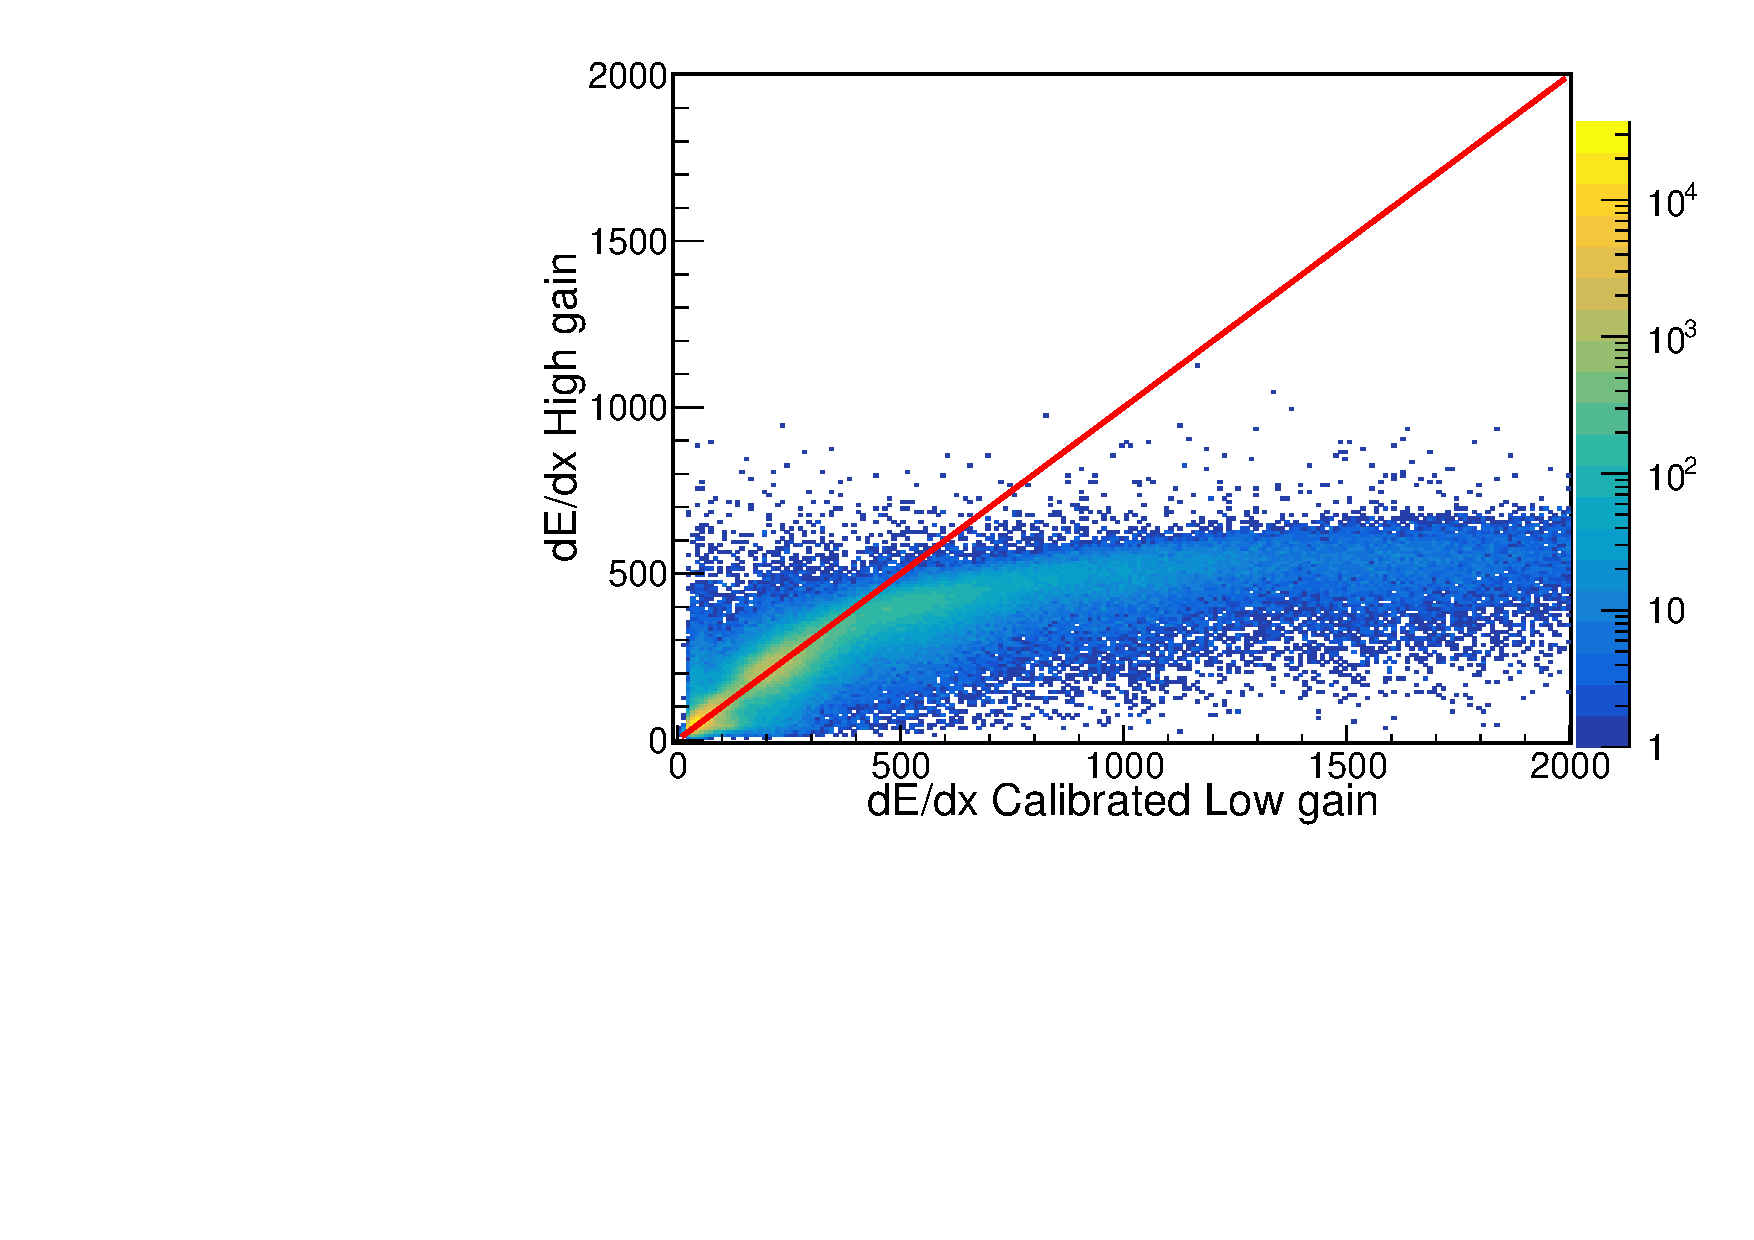
\includegraphics[width=\linewidth]{dedxcompare_nodesat}
\caption{The uncorrected high gain dE/dx vs low gain dE/dx collision data.  }
\label{fig:lowvshigh_raw}
\end{figure}
 
When plotting the raw data in figure \ref{fig:lowvshigh_raw}, the effect of saturation can be seen on the high gain channels. For signals in size below 400 ADC/mm the electronics are not saturated and therefore the high and low gain sections agree. The data starts to saturate and deviates above 400 ADC/mm in the high gain channels and eventually plateaus. Though these events saturate the high gain sections the low gain sections still have not saturated and provide the true dE/dx values. After applying the desaturation method, the correction the correlation between the high gain and low gain sections is significantly restored as seen in figure \ref{fig:lowvshigh_desat}. Judging by the data in the corrected correlation plot we believe the correction to at least about 900 ADC/mm. It seems the 1:1 correlation which was a plateau before is mostly restored and the increase in dynamic range in the high gain pads by at least a factor of 2x.  

\begin{figure}[H]
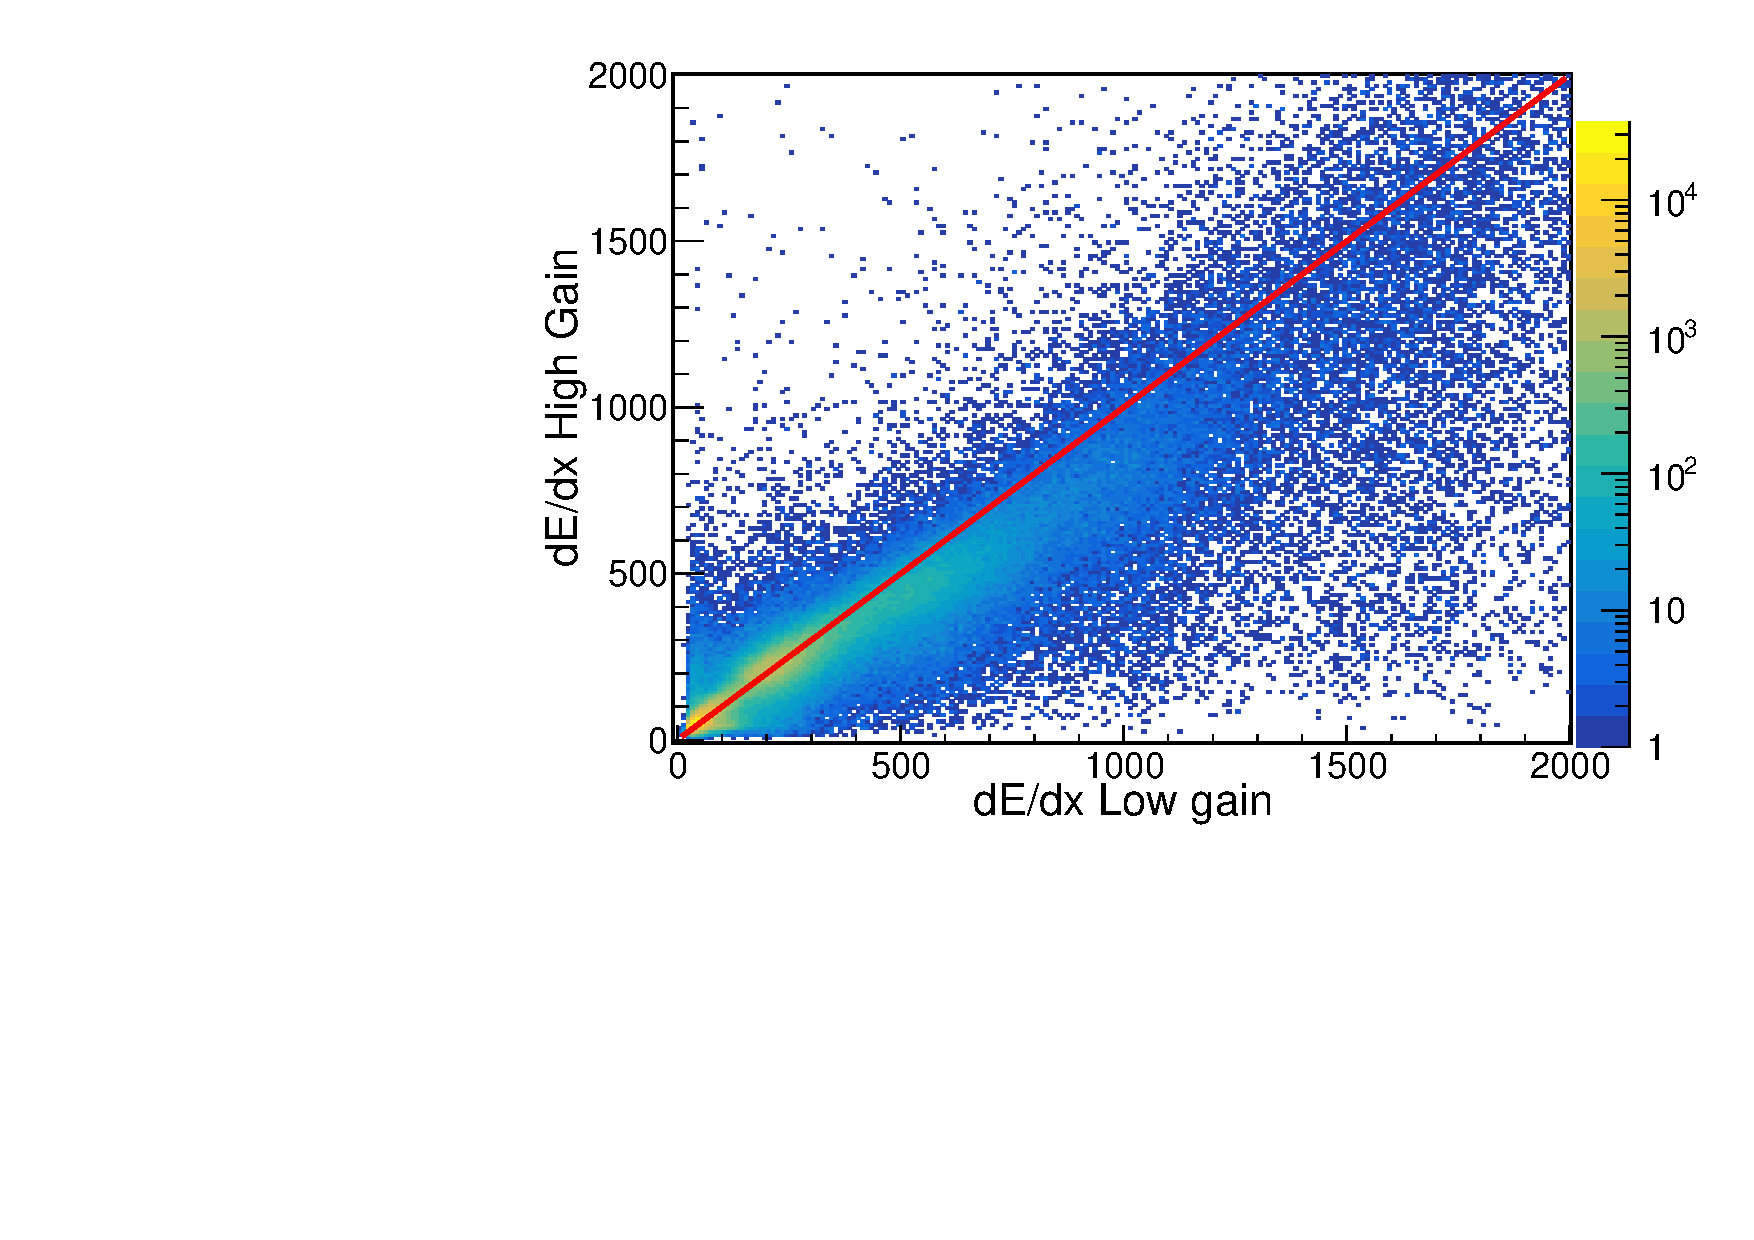
\includegraphics[width=\linewidth]{dedxcompare_new}
\caption{The corrected high gain dE/dx vs low gain dE/dx for ~??? events of collision data.  }
\label{fig:lowvshigh_desat}
\end{figure}

\paragraph{Particle Identification (PID)}

Comparing the low to high gain sections provides a direct comparison for determining the success of the extrapolation. But, the true goal of any correction would be to improve the PID. 

\begin{figure}[H]
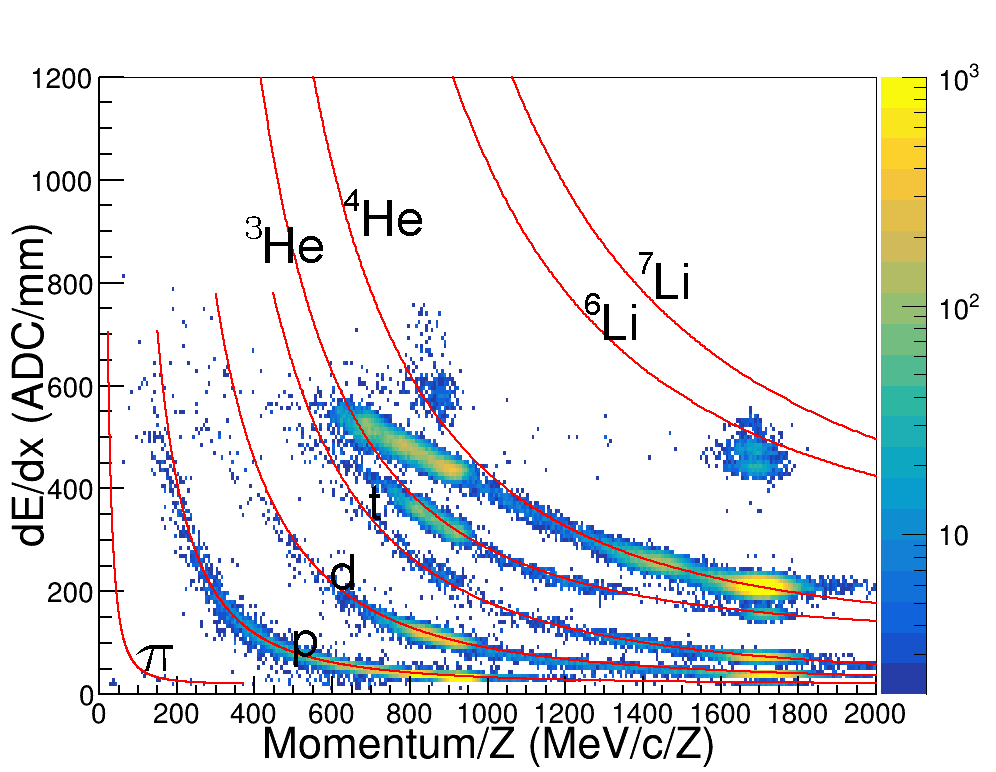
\includegraphics[width=\linewidth]{cocktail_raw}
\caption{Uncorrected cocktail data.}
\label{fig:cocktail_raw}
\end{figure}

Looking firstly at the ideal case of the cocktail beam in figures \ref{fig:cocktail_raw} and \ref{fig:cocktail_desat} we note the very clean pronounced PID lines of several particle species. Once can clearly see the three  B$\rho$ settings of the fragment separator leading to three ovals around 1700 and two near 900 [MeV/c/Z]. The tails of the PID lines leading away from these three ovals are resulting from the particle losing its initial energy by passing through the walls and other materials outside the main detector volume, therefore lowering their initial momentum. The red lines are the theoretical PID lines representing the most probable energy loss as given by Bichsel straggling functions after calibration to the experimental data. One can also get similar curves from Geant4. Looking at the uncorrected data in figure \ref{fig:cocktail_raw} we can see the effects of saturation. It seems the dE/dx values plateau and the PID lines deviate from their theoretical expectations starting around 400 ADC/mm as we also saw in figure \ref{fig:lowvshigh_raw}. After applying the desaturation method we see a stark difference in figures \ref{fig:cocktail_raw} and \ref{fig:cocktail_desat}. Most notable is the difference between He and Li particle species which suffer the most from saturation. Also a more subtle improvement of the lighter particles, (p,d,t), can also be seen in the PID values at lower momentum.

\begin{figure}[H]
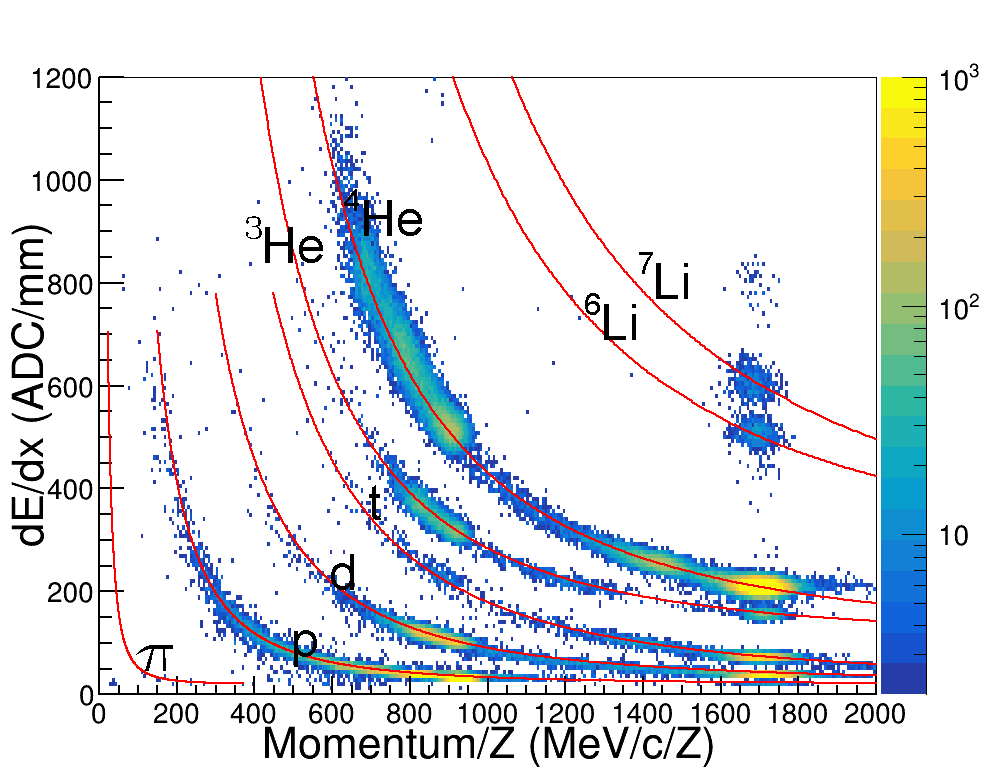
\includegraphics[width=\linewidth]{cocktail_desat}
\caption{Corrected (desaturated) cocktail data.}
\label{fig:cocktail_desat}
\end{figure}


 
Looking to the collision data in figures $\ref{fig:data_raw}$ and $\ref{fig:data_desat}$ we also see a similar result. Of course the collision data PID is much less clean than the ideal case of the cocktail beam, nevertheless we can see a similar improvement in the PID lines of the real data when comparing the raw to after the desaturation has been applied. Most notably in the separation of particle species at lower momenta. 

\begin{figure}[H]
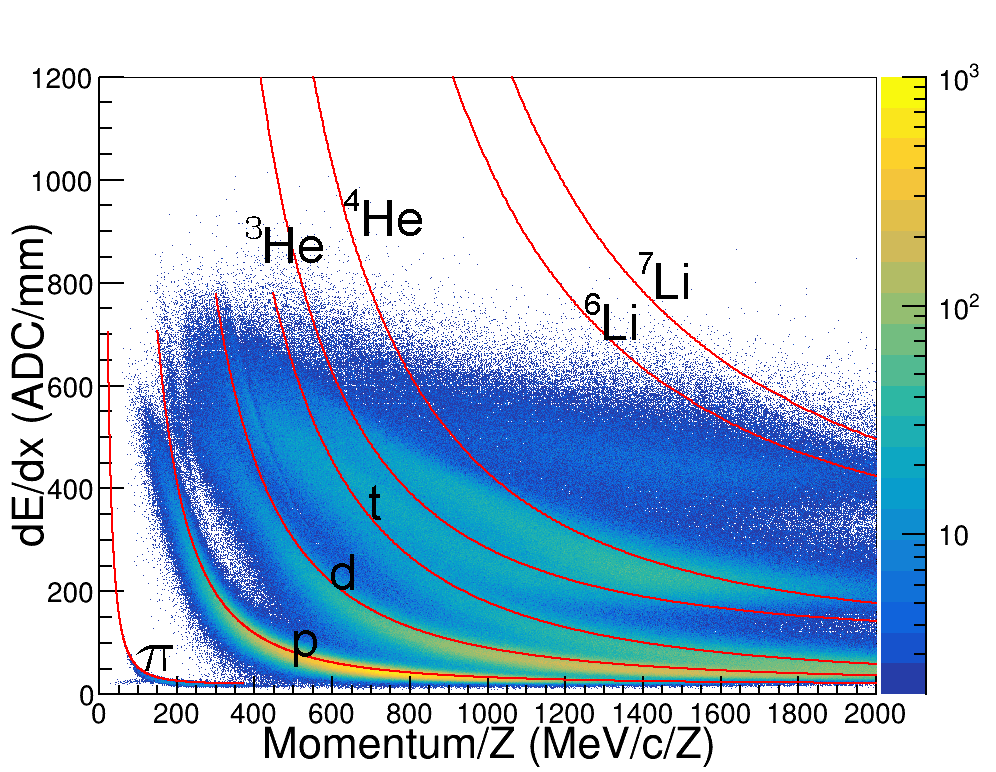
\includegraphics[width=\linewidth]{data_raw}
\caption{Uncorrected collision data.}
\label{fig:data_raw}
\end{figure}

\begin{figure}[H]
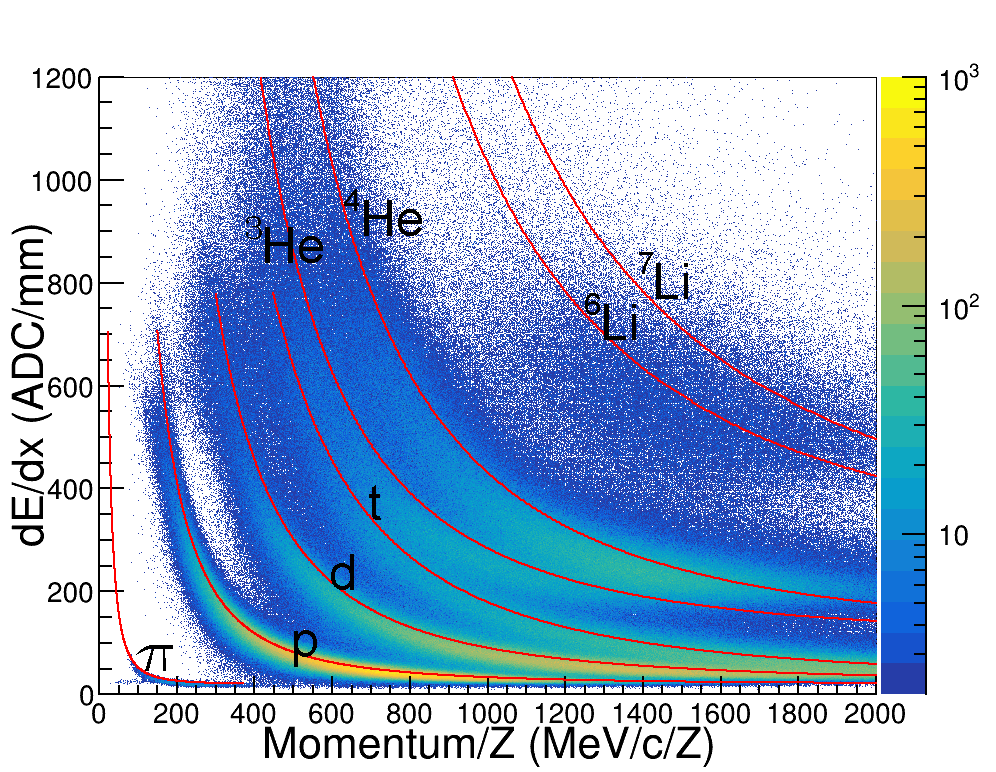
\includegraphics[width=\linewidth]{data_desat}
\caption{Corrected (desaturated) collision data.}
\label{fig:data_desat}
\end{figure}


\section{Conclusion}
The Pad Response Function (PRF) is fixed by the anode wire geometry of the TPC and an experimental PRF can be calculated from unsaturated experimental data. It is also true that for all pad charges follow this PRF independent of the initial charge of deposited on the wire. By applying a simple $\chi^2$ fit to the unsaturated tails of pad distribution, one can recover the saturated pad's charges in the middle of this distribution. We also demonstrated the success of this method by a direct comparison of dE/dx obtained in the high gain sections, to the dE/dx value obtained in the low gain sections. Also significant improvement of the PID of both cocktail calibration and nuclear collision data is seen. Using this simple method we were able to extend the dynamic range by at least a factor of 2x. 
\section*{References}

\bibliography{mybibfile}

\end{document}